\documentclass{article}
\usepackage{graphicx}
\usepackage{amsmath}
\usepackage{amsfonts}
\usepackage{bookmark}
\usepackage{booktabs}
\usepackage{exercises}
\graphicspath{ {./images/5.2} }
\usepackage{indentfirst}
\usepackage{amsthm}
\usepackage{yhmath}
\usepackage{geometry}
\usepackage{placeins}
\usepackage{csquotes}
\usepackage{pgfplots}
\newcommand*{\oldneg}{\mathord{\sim}}
\newcommand\showdiv[1]{\overline{\smash{)}#1}}
\newcommand\Mydiv[1]{%
\smash{\raise.3ex\hbox{$\big)$}}\mkern-8mu
        \overline{\enspace\strut#1}}
\setlength{\tabcolsep}{5pt}
\theoremstyle{definition}
\newtheorem{definition}{Definition}

\setlength{\parindent}{.5in}
\setlength{\parskip}{12pt}
\renewcommand{\arraystretch}{2}
\geometry{margin=1in}
\newcommand{\?}{\stackrel{?}{=}}
\pgfplotsset{width=7cm,compat=1.18}\usepgfplotslibrary{statistics}

\title{5.2 Answers}
\begin{document}
\maketitle

\section*{1}
The fucntion $y=\frac{7}{x+4}+3$ has a range of all real numbers except 3 and a domain of all real numbers except $-4$.

\section*{2}
A function $f(x)$ is defined to a rational function iff it is of the form $\frac{p(x)}{q(x)}$ where both $p$ and $q$ are polynomials. In the given example, 
$f(x)=\frac{-3x+5}{2^x+1}$. But $2^x+1$ is not a polynomial, meaning $f(x)$ is not a rational function.

\section*{9}
The graph of $g(x)=\frac{-6}{x}$ is a reflection of $f(x)=\frac{1}{x}$ across the $y$-axis, and then an enlargement:\newline
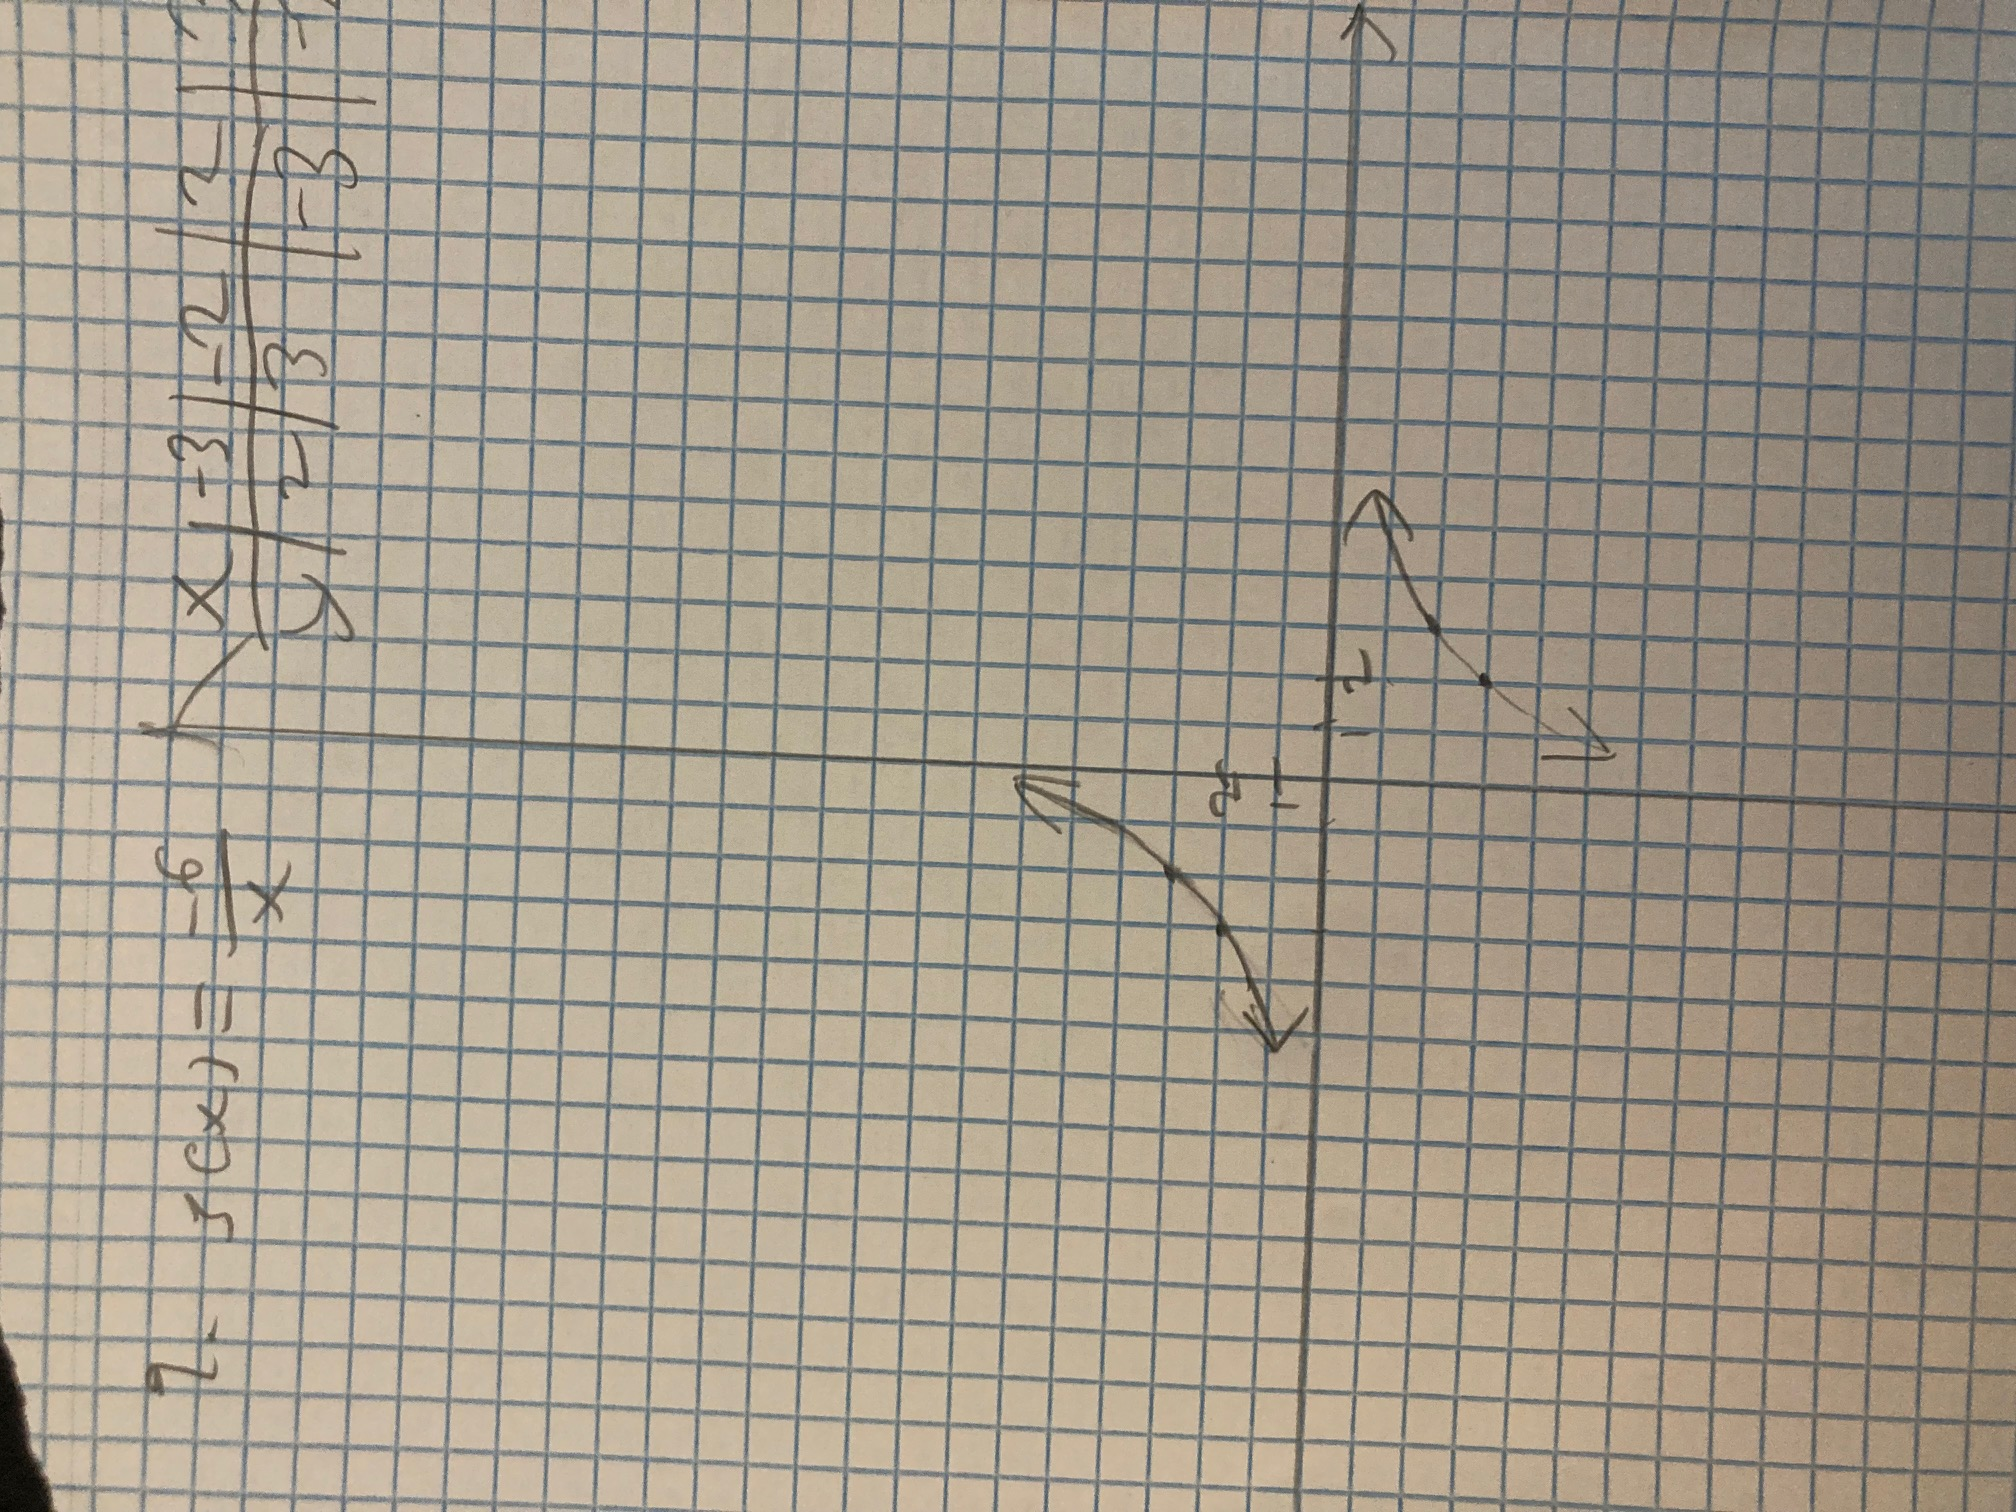
\includegraphics[width = 4in, height = 4in, angle=-90]{9}

\section*{18}
For $g(x)=\frac{-2}{x-7}$, the asymptotes are $x=7$ and $y=0$, and the domain is all real numbers other than $7$, and the range is all real numbers other than $0$:\newline
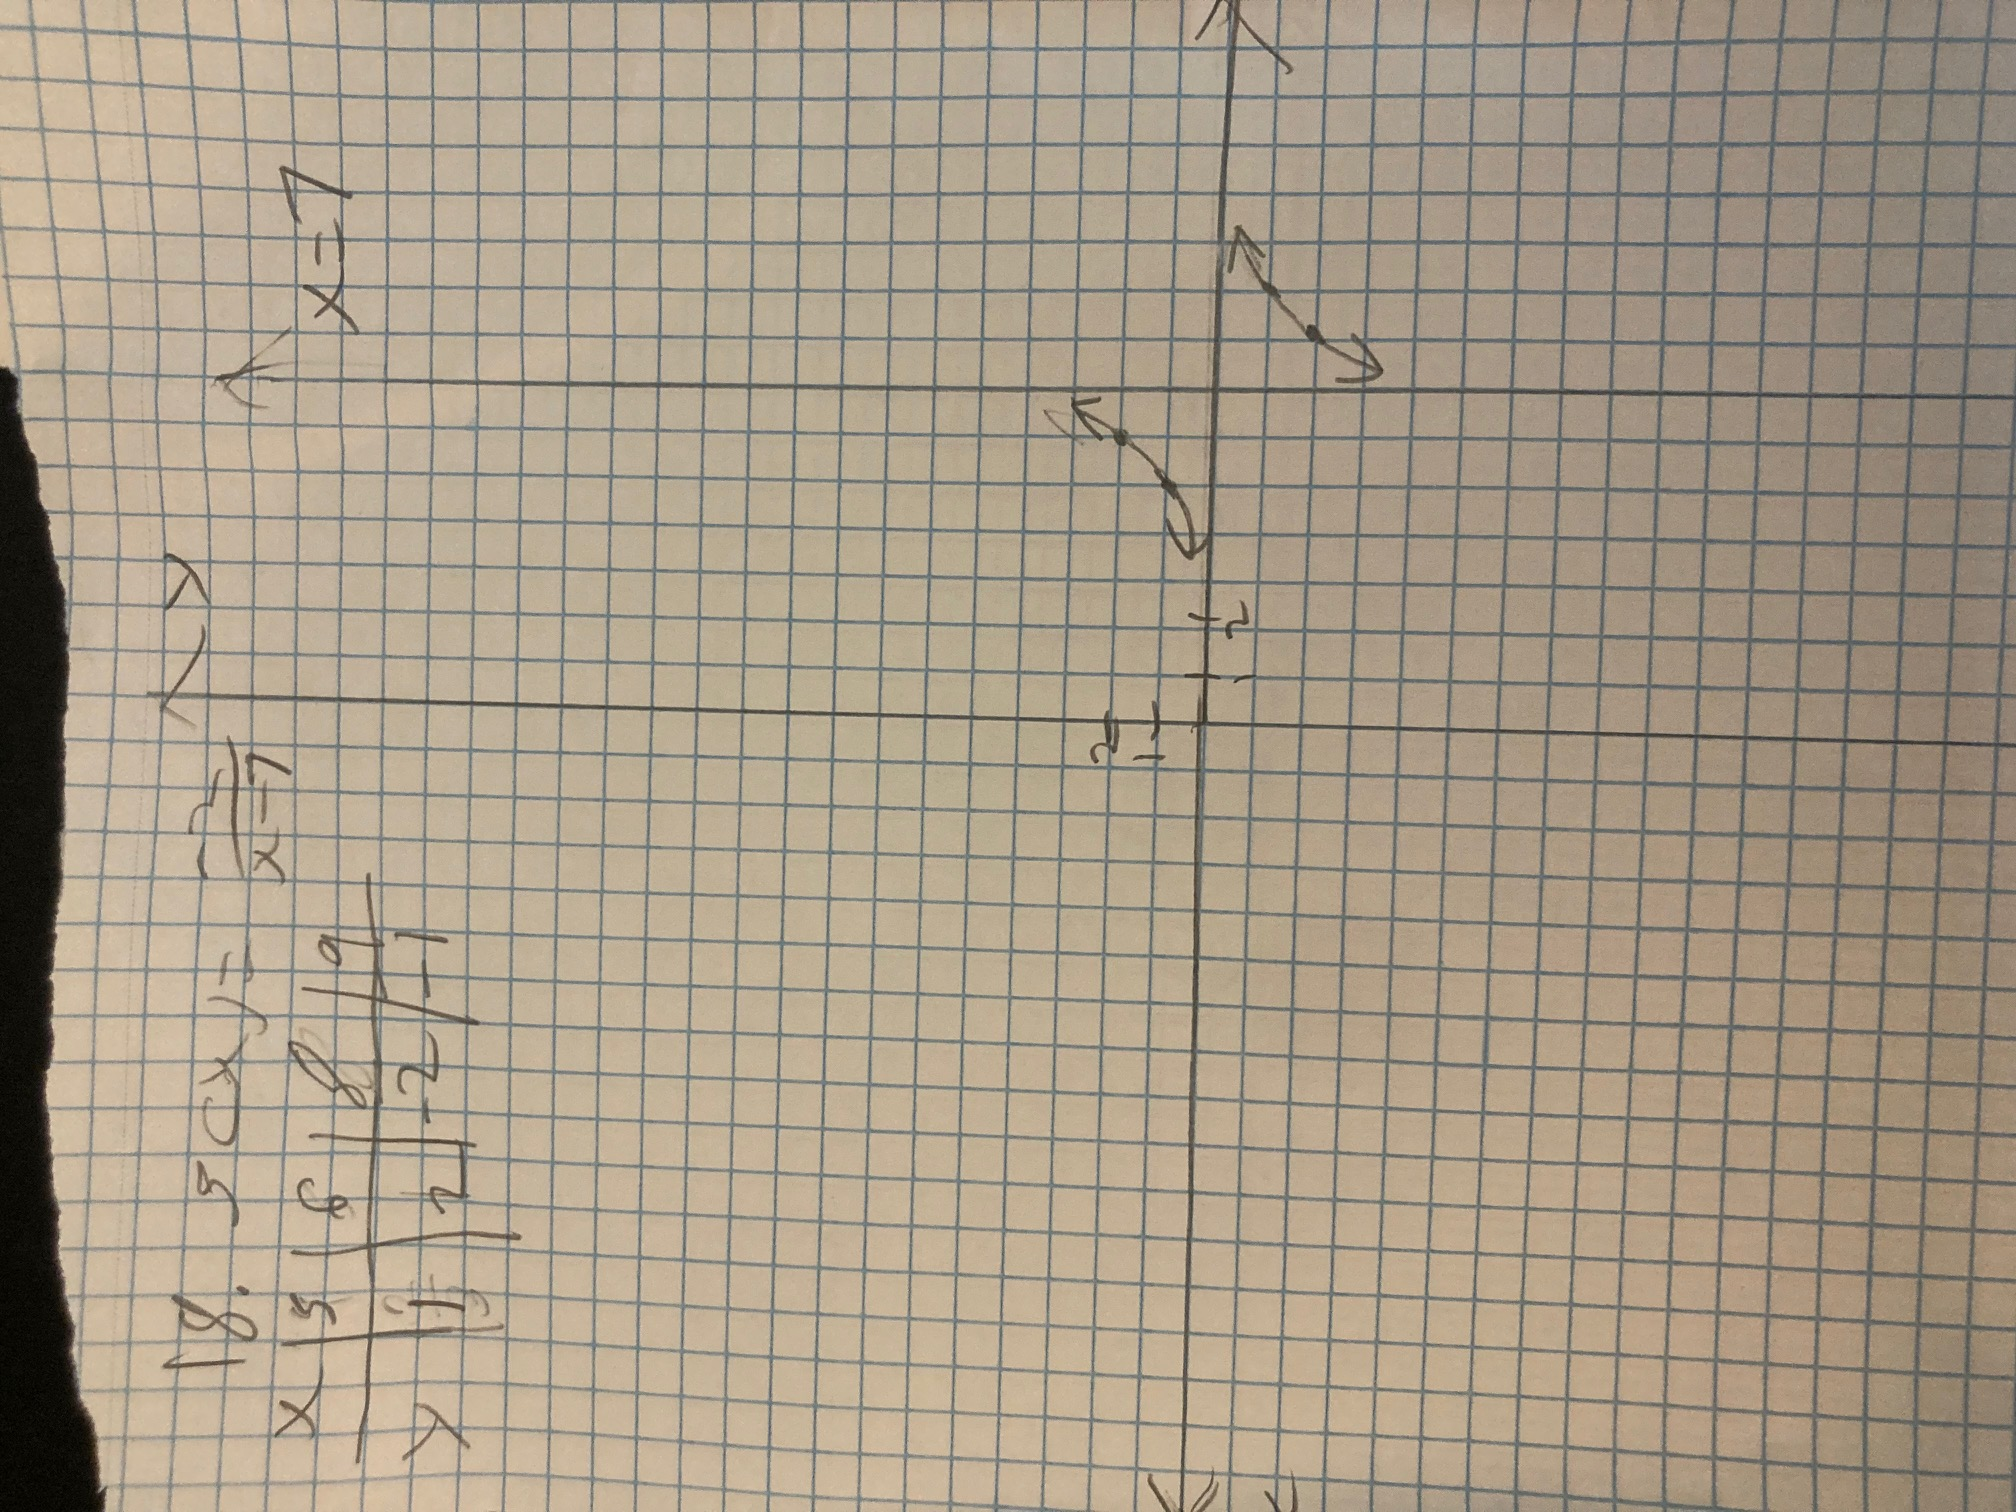
\includegraphics[width = 4in, height = 4in, angle=-90]{18}

\section*{23}
D

\section*{29}
For $f(x)=\frac{x+6}{4x-8}$, the asymptotes are $x=2$ and $y=\frac{1}{4}$, and the domain is all real numbers other than $2$, and the range is all real numbers other than $\frac{1}{4}$:\newline
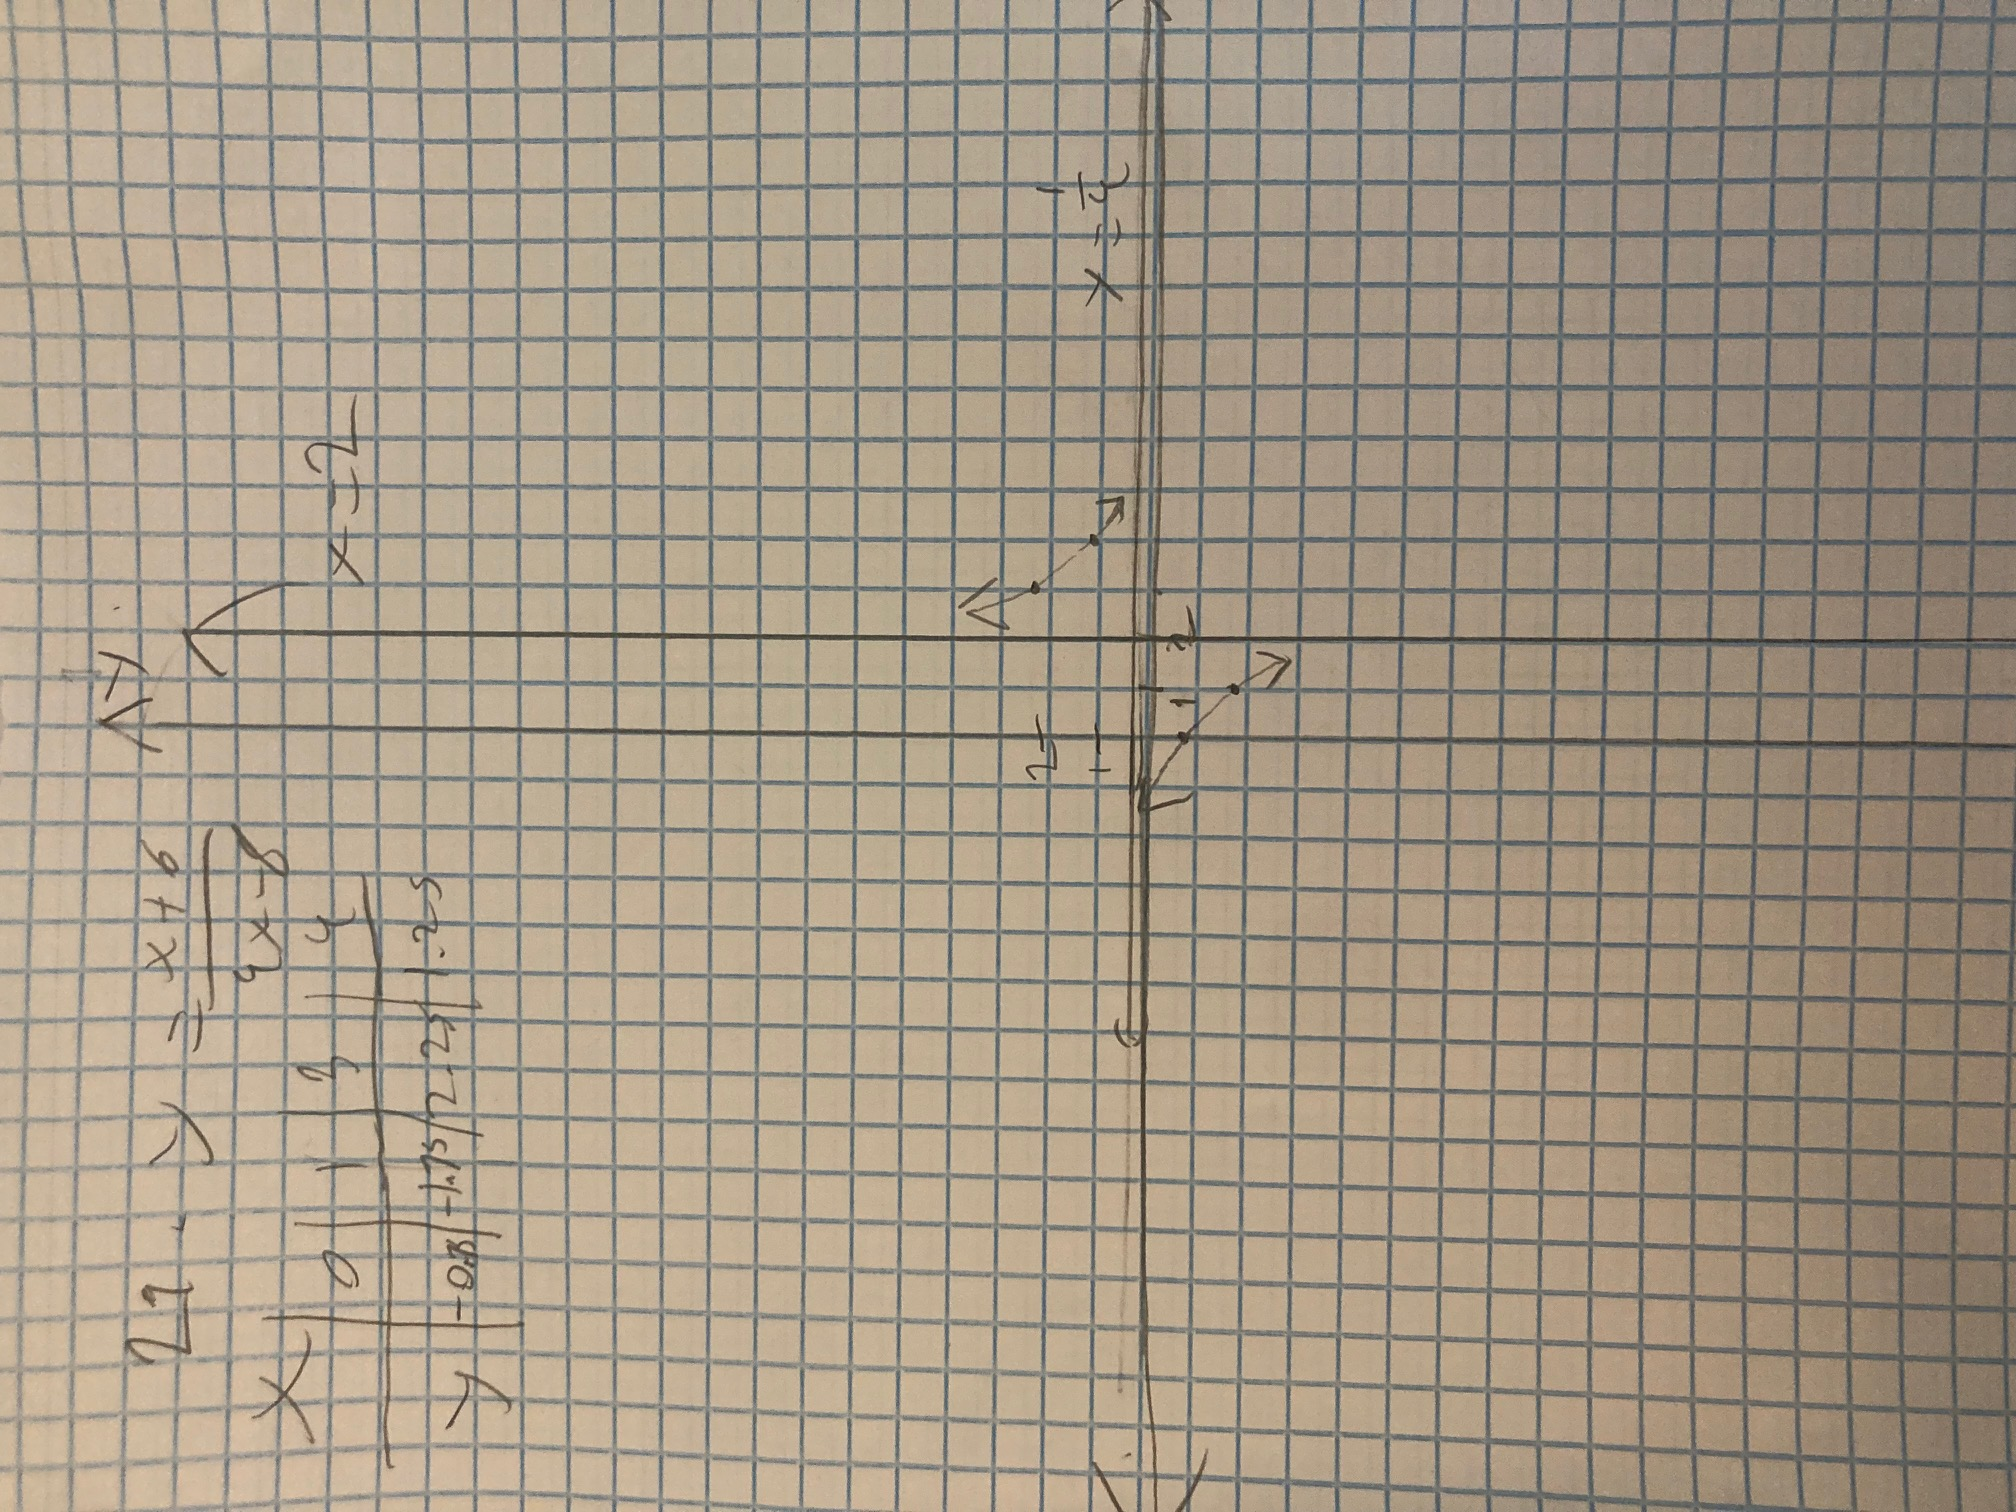
\includegraphics[width = 4in, height = 4in, angle=-90]{29}

\section*{35}
Because the domain is all real numbers except $-8$, we could have $x+8$ in the denominator. Because the range is all real numbers except 3, we could have:
\[ f(x)=\frac{2}{x+8}+3 \]

\section*{36}
\[ f(x)=\frac{a}{x-h}+k \] \[ =\frac{a}{x-h}+\frac{k(x-h)}{x-h} \] \[ =\frac{kx-kh+a}{x-h} \]

\section*{41}
(a): The equation for when the ambulance is approaching is $f_l=\frac{740\times 2000}{740+r}$ and is $f_l=\frac{740\times 2000}{740-r}$ when the ambulance is moving away.


(b): \newline 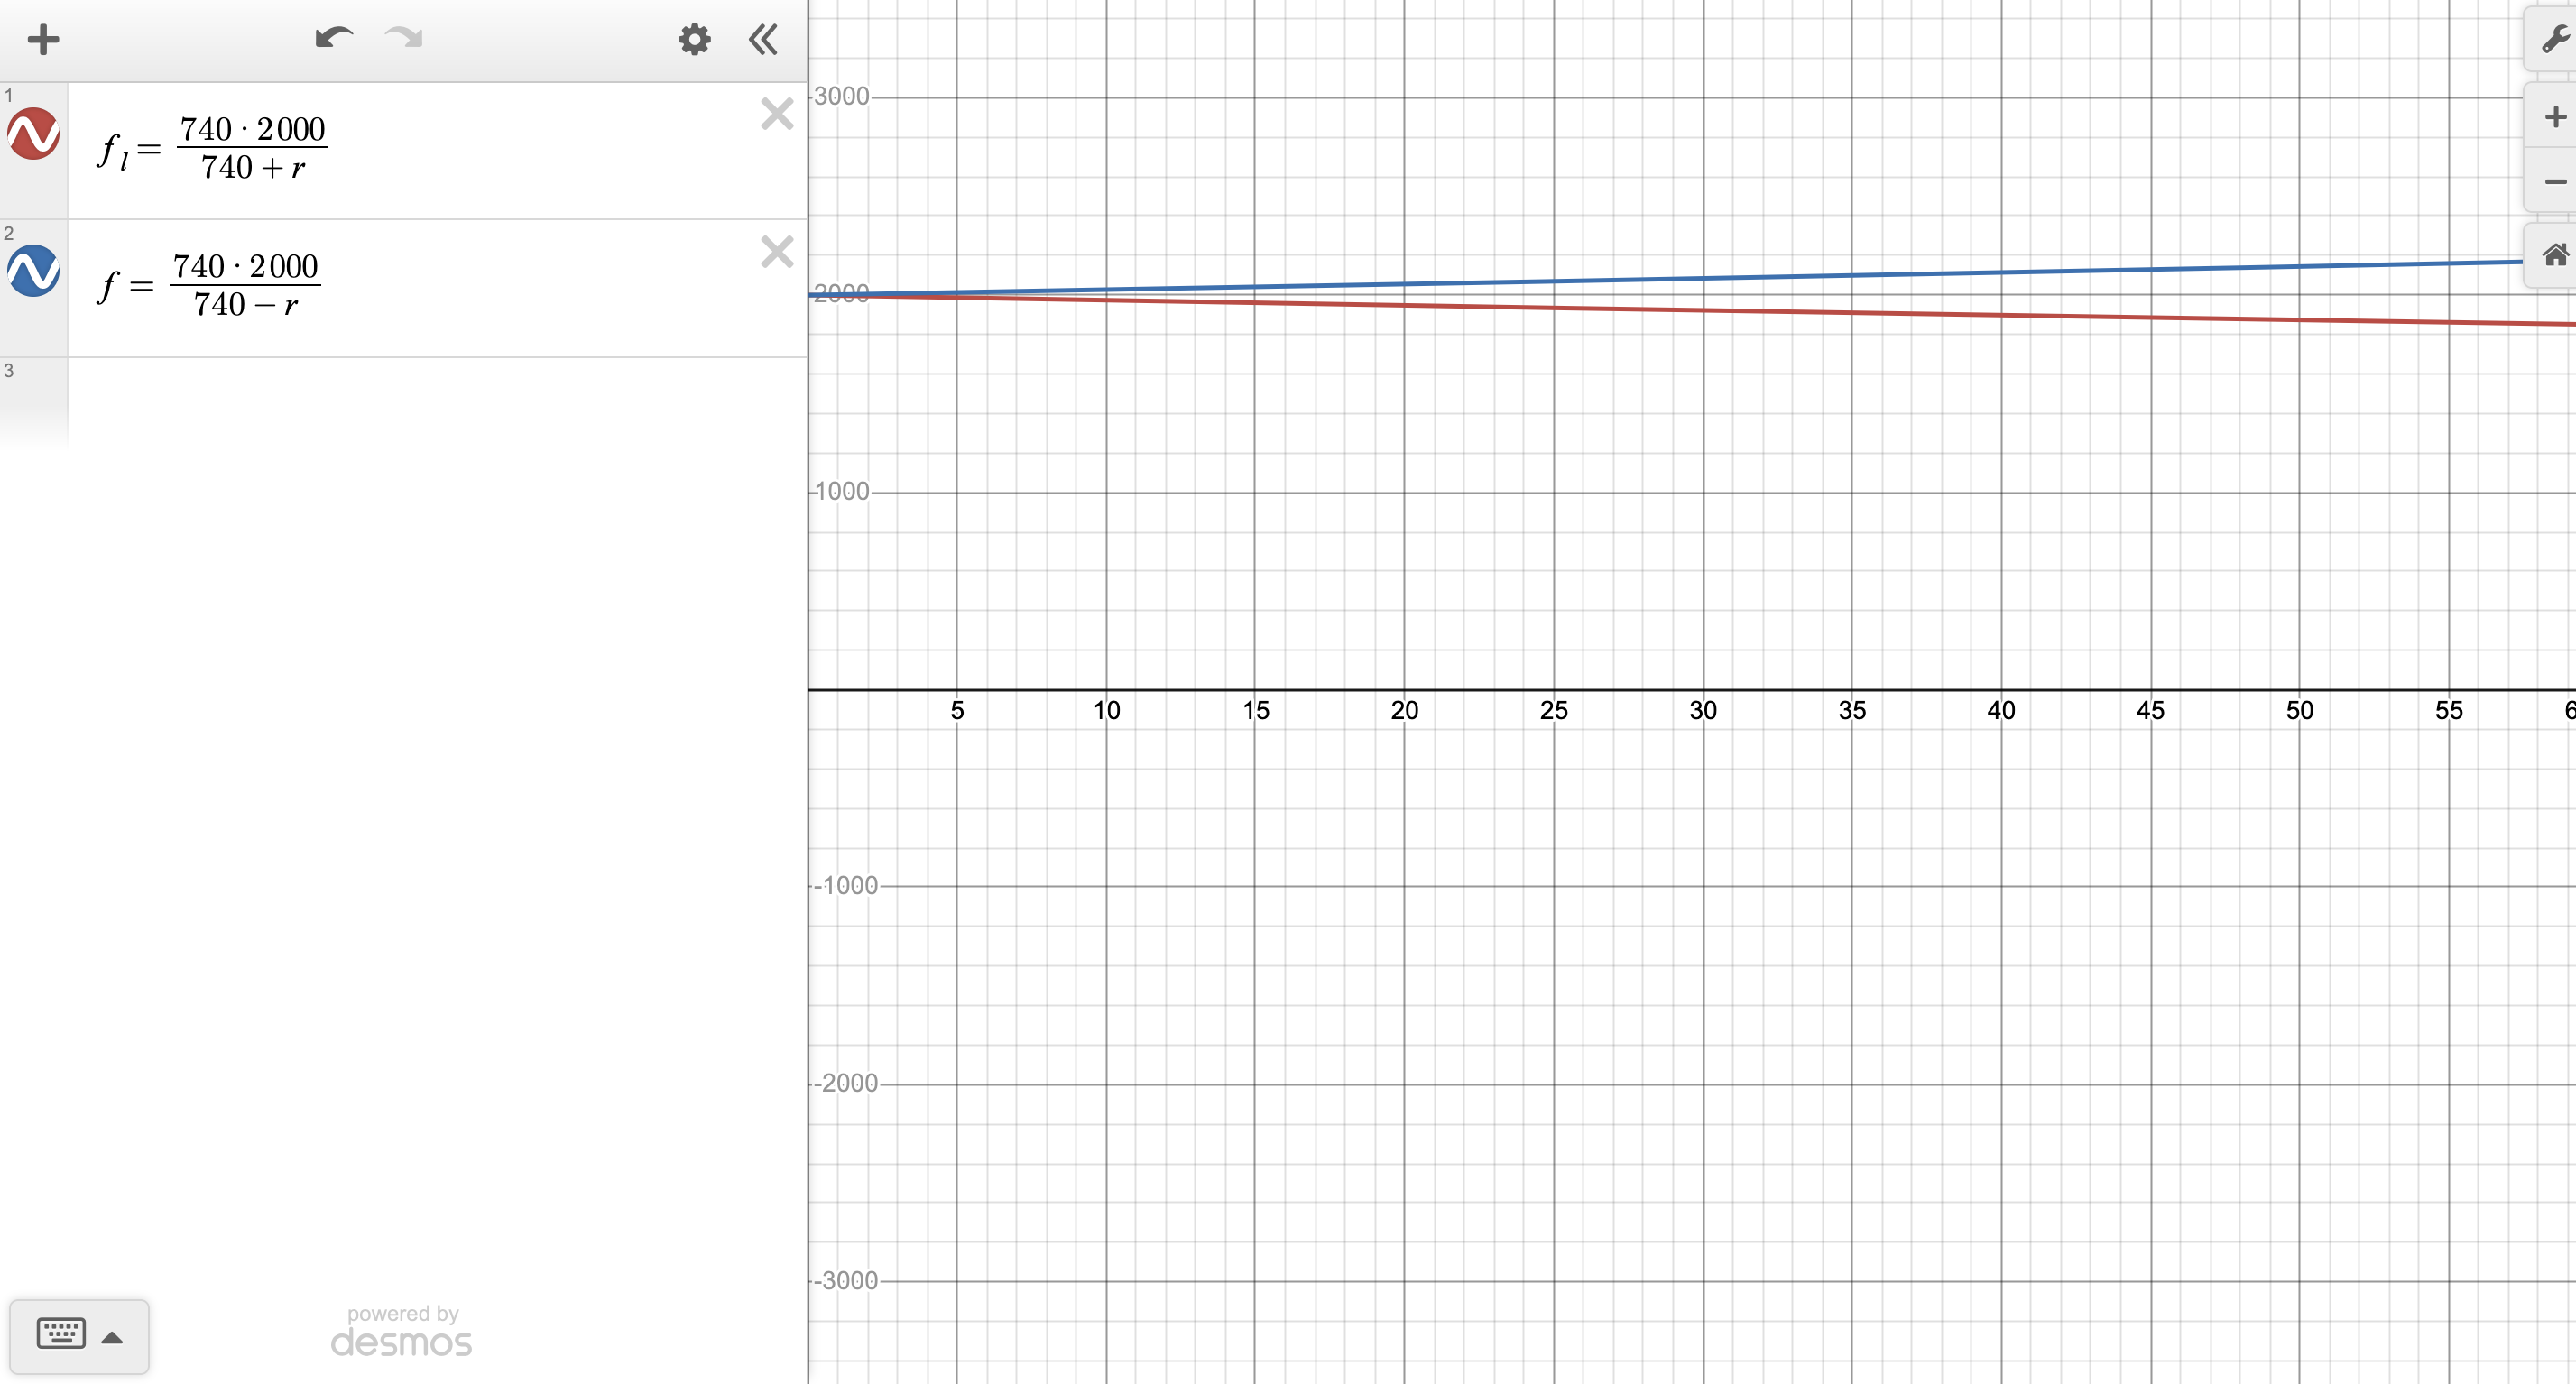
\includegraphics[width = 4in, height = 4in]{41}\newline


(c): As $r$ approaches 0, the two frequencies come closer, while as $r\rightarrow +\infty$, the frequency heard for an approaching sound source is greater than the frequency for the sound 
source moving away.

\section*{42}
An equation that can model the average speed $s$ for the entire trip is:
\[ f(x)=\begin{cases}
	t<3: & 10 \\
	t\ge 3: & \frac{10+15(t-3)}{t}
	\end{cases}
\]
A graph of the function is:\newline
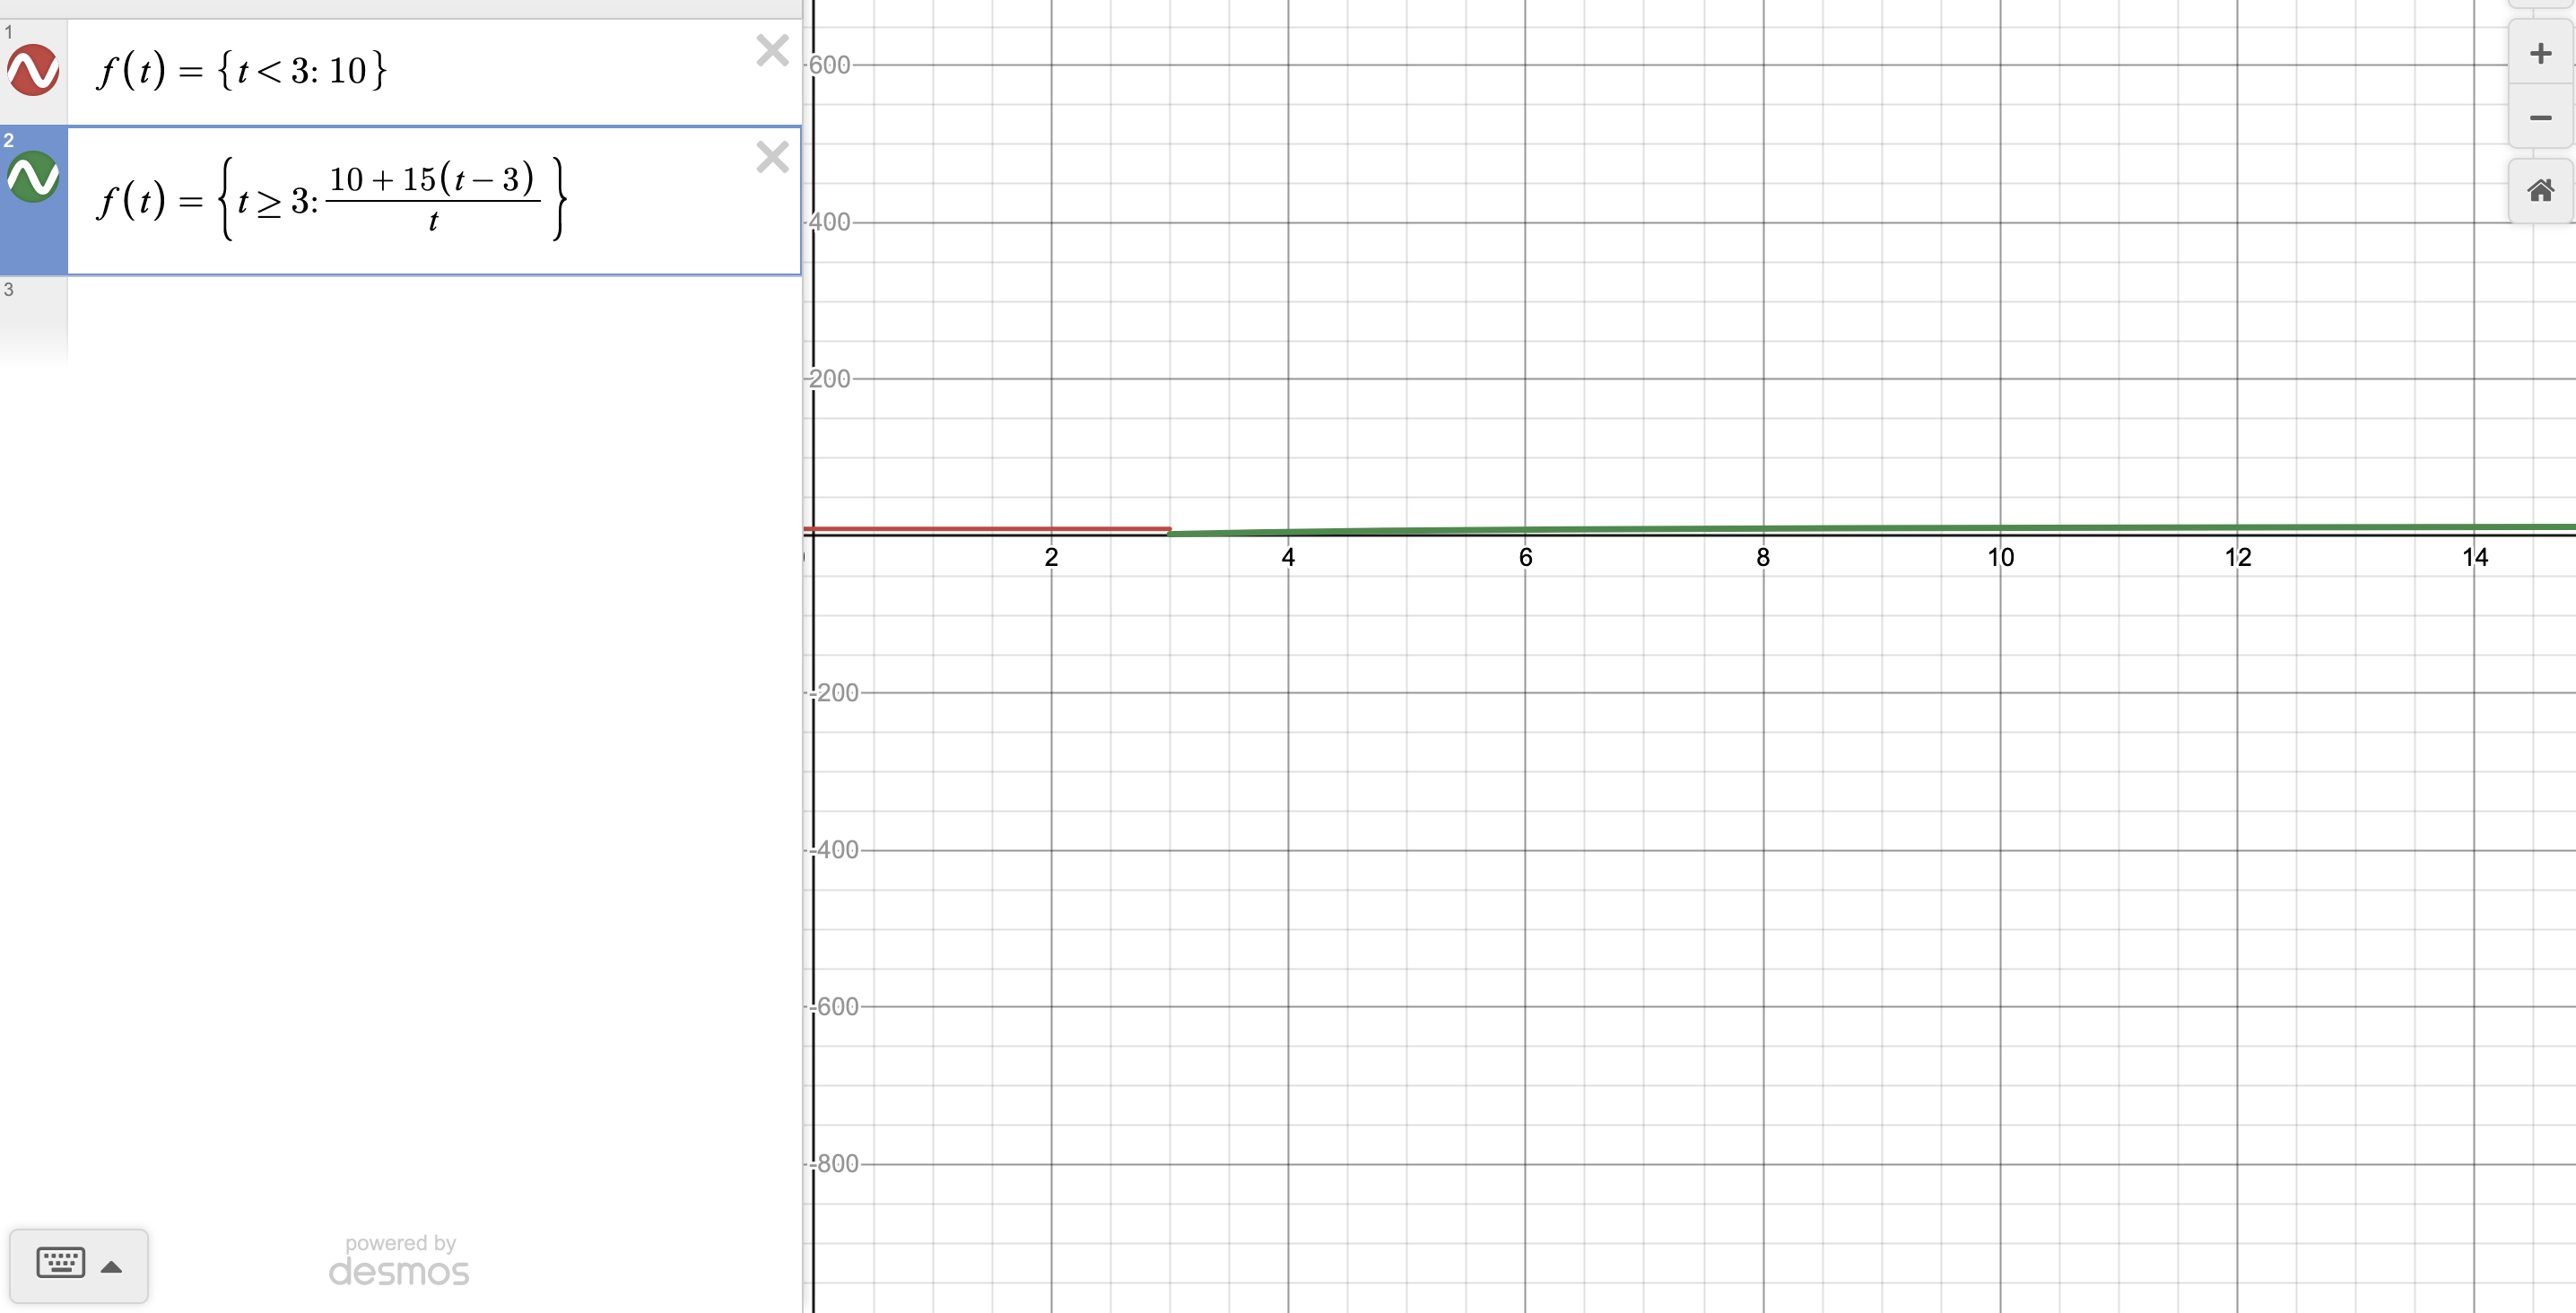
\includegraphics[width = 4in, height = 4in]{42}

\end{document}
